\section{Fitting Diffusion Barriers using Neural Network}
\label{Chap:Al/Vac:section:NN}

The computational engine that provided the energetics used to evaluate energy differences and activation barriers before and after vacancy jump in Al 7075 alloy was the implementation of \ac{DFT} together with climbing image \acf{NEB} in the \ac{VASP} software with VTST package from Henkelman's group \cite{henkelman2000climbing,henkelman2000improved}. All-electron \ac{PAW} potentials were employed for the elemental constituents with the \ac{GGA} of \ac{PBE} for the exchange-correlation energy functional, $\mu_{xc}$, and the interpolation formula of Vosko et al. \cite{vosko1980accurate}. Using plane-wave cutoff energy of at 450.0 eV, the total energy for all models of initial and final images was converged to $10^{−7}$ eV/cell. The reciprocal space of bulk supercells was sampled with (2x2x2) k-point grids. Each grid was generated using the Monkhorst-Pack scheme \cite{monkhorst1976special}. A (4x4x4) conventional supercell with a single vacancy embedded was used for these calculations. For activation barrier calculations, 5 images between relaxed initial and final images were used. A spring constant was set to 5 $\text{eV}/\angstrom^2$. The force convergence criteria for all models was set to be less than 0.05 $\text{eV}/\angstrom$. The force-based quick-min optimizer was used to make \ac{NEB} calculations stable for high local concentration cases. \cite{sheppard2008optimization}

To sample a larger potential energy landscape, our \ac{NN} model training set contains mainly two different parts, as shown in Fig. \ref{Chap:Al/Vac:fig:atomic_illu}: 1) (4x4x4) randomly generated solid-solution structures with different local concentrations around jump pairs. 2) (2x2x2) randomly generated ordered structures embedded in (4x4x4) pure Al. The first training set is good for simulating vacancy diffusion of a very early stage, during which Al alloy is in the solid-solution state. The second training set is designed to accurately describe the behavior of vacancy moving across/along the boundary between solid-solution Al and ordered phases, and moving inside the ordered phases. The atomic structures of ordered phases are chosen from proposed GP zone structures from \cite{berg2001gp} and low energy ordered $\text{L1}_\text{0}, \text{L1}_\text{2}, \text{L1}_\text{0}^*, \text{W2}, \text{CH}, \text{L1}_\text{2}^*, \text{Z1}$ structures of Au-Fe from \cite{zhuravlev2017phase} with random species perturbation. 


\begingroup
\begin{figure}[!ht]
  \centering
  \subfigure[]{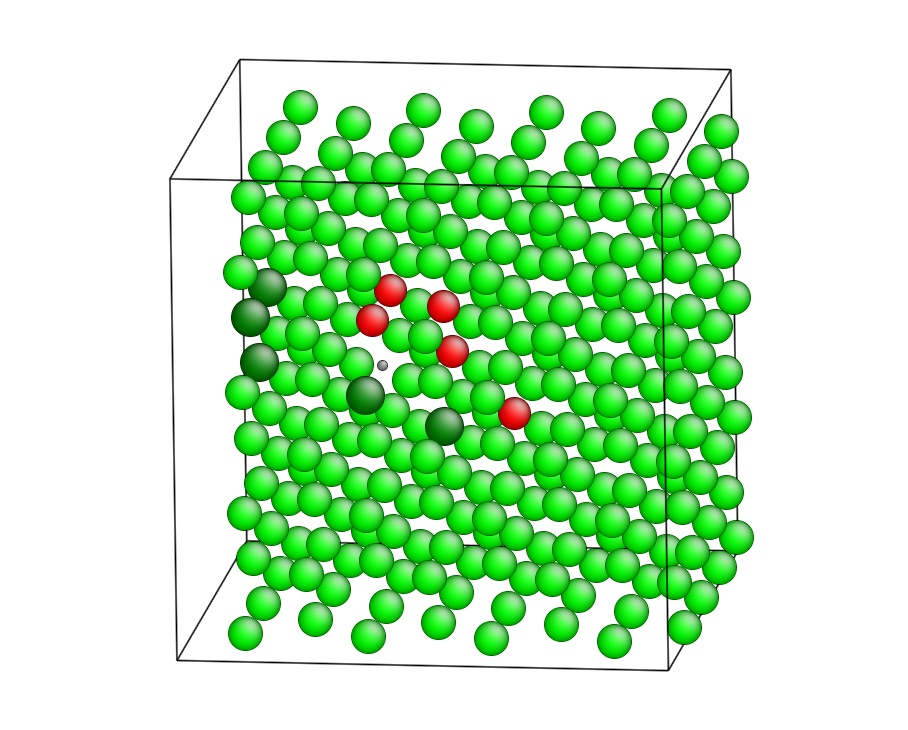
\includegraphics[width=0.49\linewidth]{Chap5/plots/ss_atomic.jpg}}
  \subfigure[]{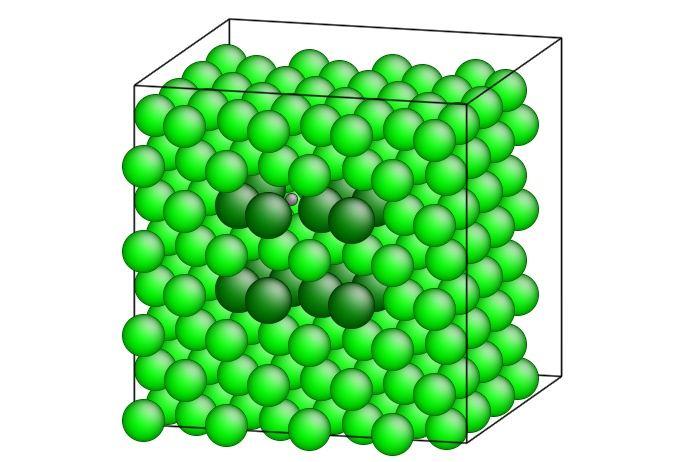
\includegraphics[width=0.49\linewidth]{Chap5/plots/ordered_atomic.jpg}}
\caption[Atomistic pictures of (4x4x4) supercells containing 256 atoms.]{Atomistic pictures of (4x4x4) supercells containing 256 atoms. (a) One typical (4x4x4) randomly generated solid-solution structure. (b) One typical (2x2x2) randomly generated ordered structures embedded in (4x4x4) pure Al. Light green, dark green, and red atoms are Al, Mg, and Zn, respectively. The small gray atom represents the location of vacancy.}
\label{Chap:Al/Vac:fig:atomic_illu}
\end{figure}
\endgroup

Many different machine learning/deep learning models are widely used, each one suitable for a different kind of problem. \cite{bartok2010gaussian,behler2011atom,szlachta2014accuracy,artrith2016implementation,mehta2014exact,artrith2017efficient} For our particular problem, the feed-forward Artificial Neural Network (ANN) is chosen, as it provides a general frame to map non-linear input (atomic species of neighboring environment) to a continuous regressor (diffusion barriers). It is well known that a sufficiently large number of hidden neurons can approximate any continuous multivariate function. \cite{hornik1989multilayer} This property gives us the most expandability of this framework when the system needs to go even further complicated in terms of the number of species considered. 

The output layer of our \ac{NN} model predicts diffusion barriers in a 1-D continuous space. The input layer is chosen to be 27 discrete numbers representing atom species, as shown in Table. \ref{Chap:Al/Vac:tab:mapping}. Among the 27 numbers, the first one indicates the type of atom that will be swap with the vacancy. The rest 26 (each atom has 12 + 6 = 18 $\text{2}^{nd}$ nearest neighbors. And both of them share 10 in common.) atoms represents the neighboring atoms of the jump pair up to their $\text{2}^{nd}$ nearest neighbors, as shown in Fig. \ref{Chap:Al/Vac:fig:2nn}. These 26 numbers are arranged in their geographical order (ascending in X, Y, and Z accordingly), so their position will always respond to the same input neuron in the \ac{NN} architecture. Besides, this cluster of 26 neighboring atoms also has 2-fold symmetry, mirror symmetry along Y-Z plane, and mirror symmetry along the X-Y plane. Therefore, for one jumping event, the diffusion barrier is taken as the average of the four symmetric configurations of the 26 neighboring atoms to have a symmetry-invariant prediction.

\begin{table}[!htbp]
\centering
\caption[Atom species encoding map for the \acf{NN} input layer.]{Atom species encoding map for the \acf{NN} input layer. Here, ``Vac'' represents vacancies.}
\label{Chap:Al/Vac:tab:mapping}
\begin{tabular}{ll}
\\
\hline
\hline
Species & Encoding  \\ \hline
Al & 1.0 \\
Mg & 2.0 \\
Zn & 3.0 \\
Vac & 4.0 \\
\hline
\hline
\end{tabular}
\end{table}

\begingroup
\begin{figure}[!ht]
  \centering
  \subfigure{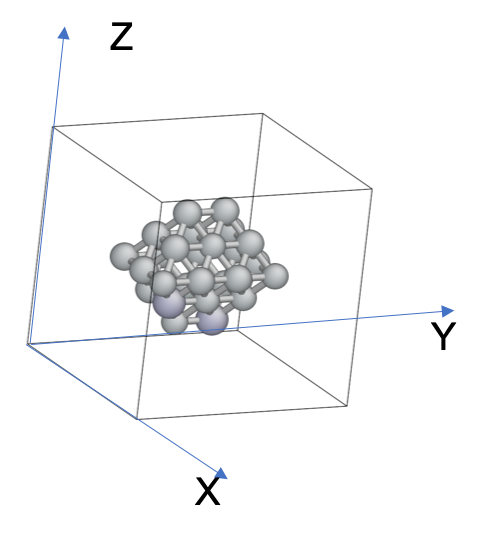
\includegraphics[width=0.5\linewidth]{Chap5/plots/2nn.png}}
\caption[Illustration of atomic structures of the $\text{2}^{nd}$ nearest neighbors surrounding the jumping pairs.]{Illustration of atomic structures of the $\text{2}^{nd}$ nearest neighbors surrounding the jumping pairs.}
\label{Chap:Al/Vac:fig:2nn}
\end{figure}
\endgroup


\newpage
\begingroup
\begin{figure}[!ht]
  \centering
  \subfigure[]{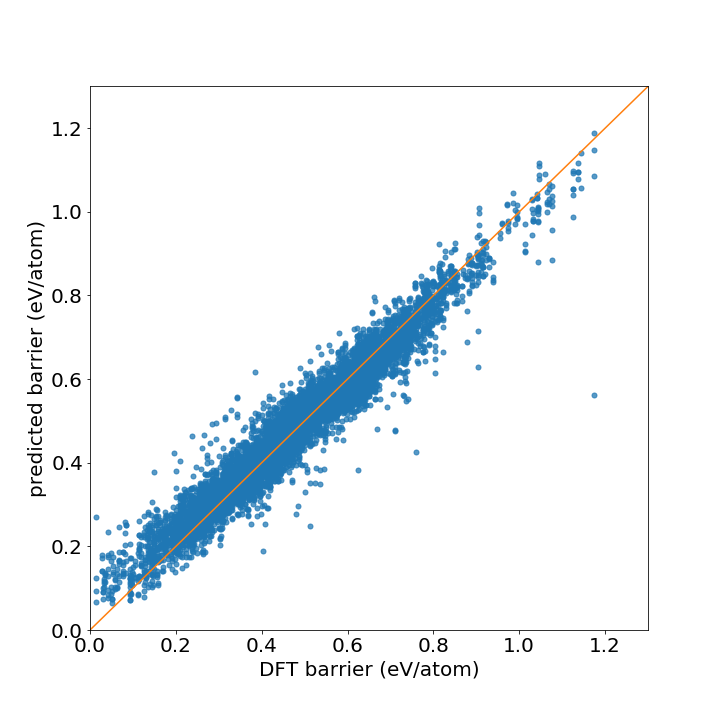
\includegraphics[width=0.49\linewidth]{Chap5/plots/total.png}}
  \subfigure[]{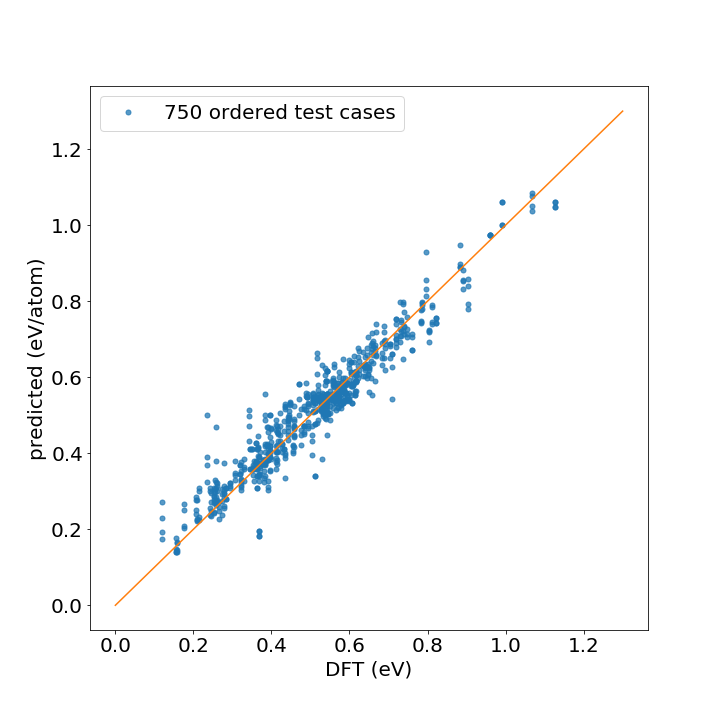
\includegraphics[width=0.49\linewidth]{Chap5/plots/fit_ordered.png}}
\caption[]{}
\label{Chap:Al/Vac:fig:fitting_all}
\end{figure}
\endgroup

